%
% File acl2021.tex
%
%% Based on the style files for EMNLP 2020, which were
%% Based on the style files for ACL 2020, which were
%% Based on the style files for ACL 2018, NAACL 2018/19, which were
%% Based on the style files for ACL-2015, with some improvements
%%  taken from the NAACL-2016 style
%% Based on the style files for ACL-2014, which were, in turn,
%% based on ACL-2013, ACL-2012, ACL-2011, ACL-2010, ACL-IJCNLP-2009,
%% EACL-2009, IJCNLP-2008...
%% Based on the style files for EACL 2006 by 
%%e.agirre@ehu.es or Sergi.Balari@uab.es
%% and that of ACL 08 by Joakim Nivre and Noah Smith

\documentclass[11pt,a4paper]{article}
\usepackage[hyperref]{acl2021}
\usepackage{times}
\usepackage{latexsym}
\renewcommand{\UrlFont}{\ttfamily\small}
\usepackage{graphicx}

% This is not strictly necessary, and may be commented out,
% but it will improve the layout of the manuscript,
% and will typically save some space.
\usepackage{microtype}

%\aclfinalcopy % Uncomment this line for the final submission
%\def\aclpaperid{***} %  Enter the acl Paper ID here

%\setlength\titlebox{5cm}
% You can expand the titlebox if you need extra space
% to show all the authors. Please do not make the titlebox
% smaller than 5cm (the original size); we will check this
% in the camera-ready version and ask you to change it back.

\newcommand\BibTeX{B\textsc{ib}\TeX}

\title{Fine-Grained Named Entity Typing beyond English Using Annotation Projection}

\author{Sabine Weber \\
  University of Edinburgh \\
  \texttt{s.weber@sms.ed.ac.uk} \\\And
  Mark Steedman \\
  University of Edinburgh \\
  \texttt{steedman@inf.ed.ac.uk} \\}

\date{}

\begin{document}
\maketitle
\begin{abstract}
Fine-grained entity typing is an important step in the construction and completion of knowledge bases from text. So far there has been no openly available system for fine-grained entity typing using the FIGER ontology \cite{ling2012fine} for languages other than English. We propose annotation projection to create a German silver annotated corpus to train a German fine-grained entity typing model. We compare the performance of the model along two axes: in-domain versus out-of-domain, and human-translated versus machine-aligned text. We propose sorting the machine aligned text by alignment quality and adding a preprocessing epoch to the training to mitigate the effects of noisy input. On a German fine-grained entity typing test set our model achieves accuracy and F1 score of level 1 label predictions within 10 percent of the English state of the art system.\end{abstract}

\section{Introduction}
%error frequency breakdown by label
%MT baseline, Take a MT model to backtranslate!
%more quantittive error analysis, error breakdown
%Accuracy? Put in precision and recall
% Put in how matches are counted, 
%precision at kn, recall at k, or does each label have a different confidence value? 
%bar plot accuracy by label


%examples from English FIGER: As a result of the Bolshevik Revolution in 1917 , the Uniechowski family lost its properties and the family was forced to move to Warsaw .      5:7     /event/protest /event/military_conflict
%The Prewitt-Allen Archeological Museum is a small archaeology museum at Corban University in Salem , Oregon , United States .   10:12   /organization/educational_institution /location

%running example: From 1997 to 2000, it had a permanent exhibition in Berlin.     In den Jahren von 1997 bis 2000 besaß es eine dauerhafte Ausstellung in Berlin. From 1997 to 2000 , it had a permanent exhibition in Berlin .   11:12   /location /location/city
%Während der gesamten parlamentarischen Republik waren die Konservativen eine der dominierenden Parteien im Kongress . 	7:8	/government /government/political_party /organization




The task of fine-grained entity typing (FET) is to assign a semantic label to a span in a text. The task is distinct from coarse-grained entity typing as done by named entity recognition systems because these systems are restricted to a small set of labels like `person', `organization', `location' and `miscellaneous' which are not very helpful for tasks that require more precise information about the entities. An example of FET can be seen in Figure \ref{figure:ex}.

%Small tree with person/location/org and the subtypes, cite Figer paper for more

Fine-grained entity typing uses a high number of types in a multilevel hierarchy, which can be seen in the label `/location/city'. In this work we use the FIGER type hierarchy which consists of two levels with 112 types in total (37 level 1, 75 level 2). FIGER types are derived from the knowledge graph Freebase \cite{bollacker2008freebase}. They are both interpretable by humans and useful in NLP applications such as relation extraction \citep{kuang2020improving}. 

\begin{figure}[t]

\centering
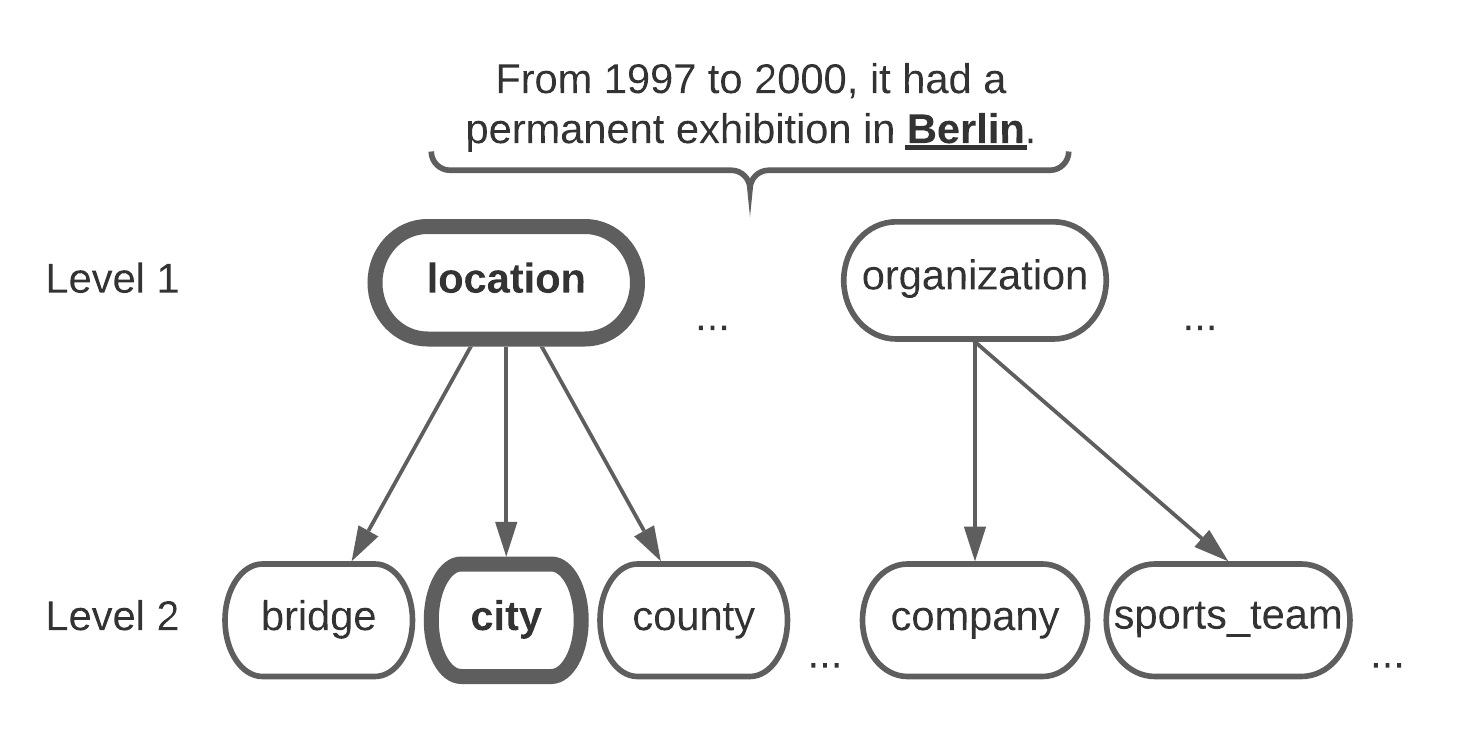
\includegraphics[width=0.45\textwidth]{diagram.png}
\caption{An example of fine-grained entity typing with the FIGER ontology. Correct entity types are highlighted.}
\label{figure:ex}
\end{figure}

Challenges in training a FET model with FIGER types arise from the high number of different and sometimes overlapping labels. An entity mentioned in a sentence can have several labels, e.g. in the sentence \textit{`As a result of the Bolshevik Revolution in 1917, the Uniechowski family was forced to move to Warsaw.'}  where `Bolshevik Revolution' is labeled both `/event/protest' and `/event/military\_conflict'. Additionally the hierarchy constraint must be obeyed: A lower label can only be predicted if it matches the higher level label (e.g. `/person/protest' would be illegal).

While there are systems for named entity recognition in languages other than English (e.g. Stanza \citet{qi2020stanza} offers NER models for 9 languages), systems for FET with FIGER types are only available in English. One of the reasons for this is the lack of FIGER annotated data in languages other than English.

While manual annotation is time consuming and expensive, the method of annotation projection \citep{Yaro:01a} uses parallel text to automatically create annotated corpora. Annotations from the resource-rich language are transferred to the resource-poor language using word alignment between translated sentences. This approach has been used for a wide variety of tasks like named entity recognition \cite{zhang2016bitext}, part-of-speech tagging \cite{huck2019cross}, lemmatization and morphological analysis \cite{nicolai2019learning}, sentiment analysis \cite{kajava2020emotion}, discourse parsing \cite{sluyter-gathje-etal-2020-shallow}, relation extraction \cite{kim2010cross}, AMR parsing \cite{damonte2018cross} and semantic role labeling \cite{pado2009cross}. To the best of our knowledge, it has not been applied to fine-grained named entity typing before. 

We use English-German parallel text and the FIGER type ontology \cite{ling2012fine} as a proof of concept that creating FET corpora via annotation projection is possible. We choose German because the availability of high-quality translation data as well as the machine aligned and therefore noisy WikiMatrix corpus \cite{schwenk2019wikimatrix} allows us to compare which role data quality plays for our approach.

We use a four step process, illustrated in Figure \ref{figure:cut}. First we use automatic named entity recognition to recognize named entities in the English half of our parallel corpora and then we use the state of the art English FET model by \citet{ChenCD20} to assign FIGER types to the entities. We then project the labels onto the German half of the corpus. The output of this process is a German corpus annotated with FIGER types.

We exchange the contextualized word embeddings in \citet{ChenCD20}'s model to adapt it to training with German input data. We also add a preprocessing epoch to the training to mitigate noise in the machine aligned input data. 

We have created a human annotated German FET test set for the domains of Wikipedia and news text, \footnote{We will release these data sets on github.} that we test our German FET models on. We treat the state of the art system by \citet{ChenCD20} trained on the 2 million sentence English FIGER data set as an upper bound for the performance we can reach using annotation projection. Our results show that training with a relatively small (200K sentences) high-quality German data set created from machine aligned data achieves results within 10 percent of accuracy and F1 score of this upper bound. We also show that domain differences (in our case Wikipedia and news text) have a significant impact on the quality of the training corpora created with annotation projection.

\section{Related Work}
\textbf{English FET} In recent years, there have been a variety of approaches advancing the state of the art in English FET using the AIDA, BNN, OntoNotes and FIGER ontologies \citep{ChenCD20, dai2019improving, lopez-etal-2019-fine}. They build on advances of contextualized word embeddings \citep{Peters:2018, conneau2019unsupervised} to generate powerful entity encodings that are then used to train a classifier. Each of the ontologies comes with a human annotated data set. We chose FIGER because of its large type set and its wide application in NLP tasks \citep{hosseini2018learning}.

\textbf{Multilingual FET} There are only few papers that consider the task of FET in other languages. \citet{lee2020chinese} and \citet{van2017multilingual} collect their own data sets from human annotations for Chinese, Spanish and Dutch. Our approach is different because we do not collect human annotations but rather work only with corpora and tools that are already available, e.g. Stanzas NER component \citet{qi2020stanza} and the WMT corpus \citep{barrault2019findings}.

\citet{yaghoobzadeh2018multi} use multi-view learning to do FET with FIGER types on 10 languages with the application of knowledge base completion. Their method operates only on entities as they appear in knowledge bases, and not entities in the context of a natural language sentence. Therefore their task is distinct from our work that uses entities in sentences as an input. For example, a line in their data set is made up of the entity `County of Flanders', its translation into other languages and the FIGER type `/location/county', while in our data set each entity appears in a sentence context e.g. \textit{`The County of Flanders was a historic territory in the Low Countries'}. In contrast to our task, they do not cover differences in surface forms of an entity (e.g. both "ex-president Obama" and "Barack Obama" refer to the same entity), but depend on disambiguating preprocessing, which makes their task easier than ours.

Two German entity typing corpora have been released recently by \citet{ruppenhofer2020fine} and \citet{leitnerdataset} consisting of annotated text from biographic interviews and German federal court decisions. \citet{ruppenhofer2020fine} extend the OntoNotes type set while \citet{leitnerdataset} introduce a new type system that is specific to the law domain. The German corpora we create via annotation projection differ in their domain (Wikipedia and news text) and in the used type system (FIGER types). By using unmodified FIGER types we ensure compatibility with downstream tasks like knowledge graph alignment across different languages.

\textbf{Annotation Projection} Annotation projection \citep{Yaro:01a} has been used for a wide variety of tasks, although it has not been applied to FET before. There exist a variety of systems that do word alignment, e.g. the Giza++ statistical machine translation suite \cite{och03:asc}, fast\_align \cite{dyer2013simple} or ZAP \cite{zap:2020}. Recent approaches use multilingual BERT and modifications of the transformer architecture to advance the state of the art in this task (e.g. \citet{nagata2020supervised, chen2020accurate}). 

\section{Method}
\subsection{Hierarchical Fine Grained Entity Typing}
We use the hierarchical typing model of \citet{ChenCD20} and train it on English and the German data. Both the entity and its context are encoded using contextualized word embeddings. For each type of the FIGER ontology the model creates a type embedding. The concatenated entity and context vector are passed trough a 2-layer feed-forward network that maps into the same space as the type embedding. The inner product between the transformed entity and context vector and the type embedding is calculated as the score. For further model details refer to \citet{ChenCD20}.

Although \citet{ChenCD20} report that ELMo contextualised embeddings \citep{Peters:2018} work better for FET than BERT \citep{devlin-etal-2019-bert}, we found this effect to be relatively small on the FIGER data set, with 4\% lower overall accuracy but 1\% higher overall F1 score when exchanging ELMo embeddings for RoBERTa\citep{conneau2019unsupervised}. We use RoBERTa because this enables us to use the same underlying word embeddings for both our German and English models, which makes their results more comparable. It also opens up the possibility for multilingual models as an avenue for future work.

%Following \citet{ChenCD20}'s method our model differs from previous FET approaches that treated labels independently by explicitly incorporating the hierarchical relation of types: a higher level type like `/location/city' will only be predicted if the model is confident of the lower level type `/location'. To do this, we use a margin loss parameter that is set higher for the coarser levels of the hierarchy and lower for the finer grained parts of the hierarchy. During test time the model also filters out any type predictions that violate the hierarchical constraint (e.g. a prediction like level 1 `/location', level 2 `/artist'). This imporves precision at the cost of recall, a trade-off that we will discuss in more detail in section 6. 



\begin{figure}[t]

\centering
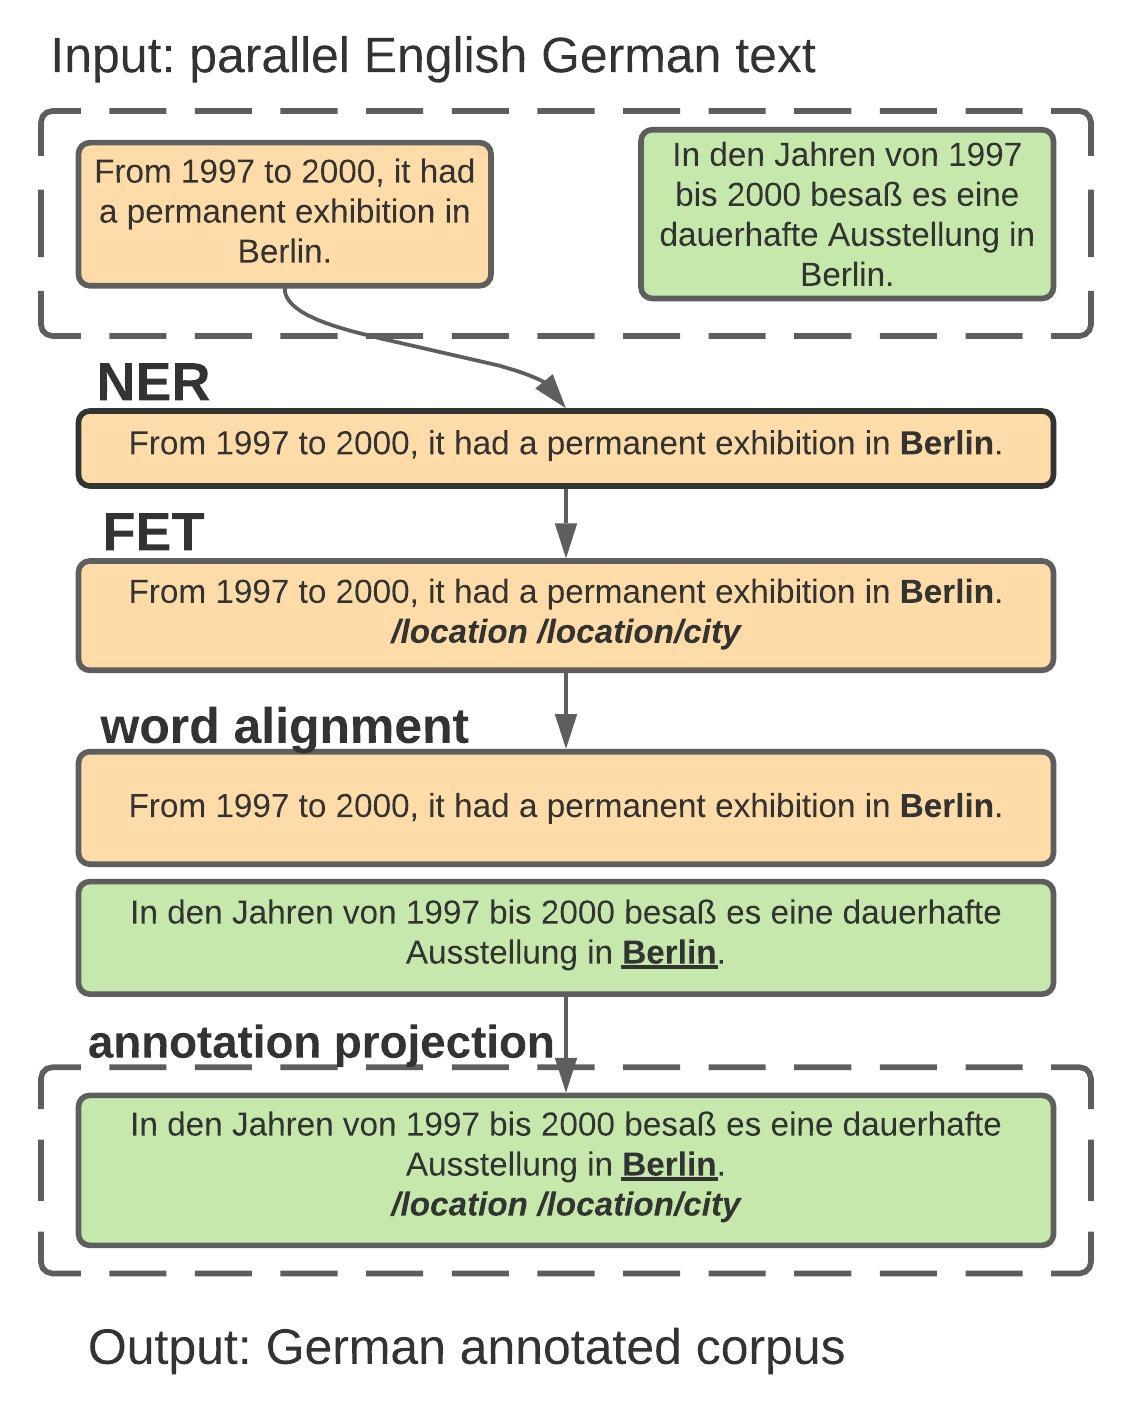
\includegraphics[width=0.45\textwidth]{annotation1.jpeg}
\caption{Our annotation projection setup uses parallel text and an automatic named entity recognition component to generate an annotated corpus in German.}
\label{figure:cut}
\end{figure}

\subsection{Annotation Projection}
ZAP \cite{zap:2020} is a framework for projection of linguistic annotation in parallel corpora. While fast\_align and Giza++ are language agnostic, ZAP provides a specifically trained model for English-German word alignment using probabilities computed for large-scale parallel corpora. We use ZAP only for word alignment and use our own code (which we will release on github) to filter out alignment errors and to transfer FIGER types from English to German named entities. 



\section{Experimental setup}
\subsection{Data sets}
\textbf{English FET training data} To train the English FET system we use the English FIGER corpus as described by \cite{ling2012fine}. Because the FIGER types are derived from the type hierarchy of the knowledge graph Freebase \citep{10.1145/1376616.1376746}, the authors linked entities found in Wikipedia to Freebase. This way they could pair the entities in a Wikipedia sentence to their respective types. The data set consists of 2 Million sentences. An example of the format of the annotation can be found in the lowest box of Figure~\ref{figure:cut}.





\textbf{English-German human translated data} During annotation projection we use an automatic word alignment system (ZAP, see section 3.2) to match a named entity in an English sentence to the German translation of the entity in a German sentence. To do this, sentence level parallel data is necessary. We compare two different sources of parallel sentences: human translations and automatically aligned text. For the human translations we took the News Commentary part of the WMT corpus \cite{barrault2019findings}. The corpus consists of 329,506 English sentences (commentary to news articles) and their German translations. 

We choose this corpus for the high quality of translations (as compared to text crawled from the web) and the more similar domain to Wikipedia (as compared to parliamentary debates from the Europarl corpus).

The News Commentary corpus belongs to a different domain than the English FET training data, which is built from Wikipedia. After the preprocessing and annotation projection steps described in 4.3 and 4.4 we obtain a German annotated data set of 500,000 sentences, which we call \textbf{German News}.

\begin{figure*}[h!]%
    \centering
    \subfloat{{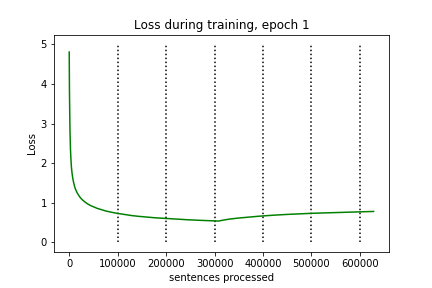
\includegraphics[width=0.45\textwidth]{loss.png} }}%
    \qquad
    \subfloat{{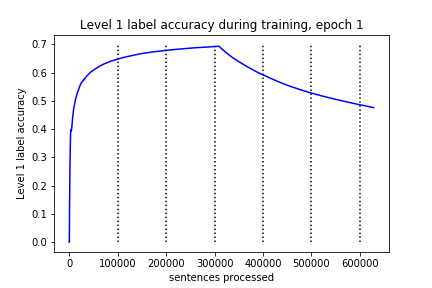
\includegraphics[width=0.45\textwidth]{l1.png} }}%
    \caption{Loss rises and level 1 label accuracy deteriorates as the quality of samples gets worse towards the end of the automatically aligned and sorted corpus. The graphs show a cut-off point at approximately 300 thousand sentences. We use this information to select a high-quality slice of the corpus to train our system.}%
    \label{fig:loss}%
\end{figure*}


\textbf{English-German machine aligned data} As a second source of parallel English-German sentences we use the WikiMatrix corpus by \citet{schwenk2019wikimatrix}. The authors mined 1,5 Million parallel sentences by creating a multilingual sentence embedding space and identifying translations of sentences using their distance in the embedding space. They used language identification tools to avoid retrieving similar sentences from the source language or translations in languages other than the target language. The corpus is sorted by the confidence value of the alignment algorithm, putting high confidence aligned sentences at the very beginning of the corpus and lower confidence sentences at the end. 

High-quality alignment is important for annotation projection. If the alignment is noisy the chances are high that the named entity in the sentence is misaligned and the projected type label will not match the word that it gets assigned to. We discover that the ordering of the WikiMatrix corpus is important for the mitigation of noise when training our German FET system which we will discuss further in section 4.3.

The WikiMatrix corpus was created for and evaluated on machine translation. Unlike the news corpus described earlier, the text in this corpus is in the same domain as the English FET training data. After preprocessing and annotation projection we obtain a data set of 600,000 sentences, which we call \textbf{German Wiki}.

We shall release all of our German training data alongside the label distribution numbers and preprocessing code on github.



\subsection{Preprocessing}
A diagram of our pipeline can be seen in figure \ref{figure:cut}. To annotate the English halves of our parallel corpora with FIGER types preprocessing is necessary. Due to its automatic creation the WikiMatrix corpus contains a small amount of German sentences in its English half and English sentences in its German half. We remove these by discarding the first 5000 sentences (for more details see appendix section A). 

%put the NER part in the method section, describe input
%make clear in the related work that the named enity needs to be annotated
%at test time we also need a ner system
To enable annotation by the English FET system, we run a named entity recognition system over the English input sentences (see the second box of Figure \ref{figure:cut}). We used the NER component of Stanza \cite{qi2020stanza} for this task. We then use the English FET model to assign FIGER types to the named entities (see the third box of Figure \ref{figure:cut}). The FET model only annotates one entity per sentence. Sentences that contain more than one named entity occur multiple times in the English input, so that each entity receives an annotation.




\subsection{Annotation projection and training with noise mitigation }
We use ZAP to obtain a word alignment between the English and German halves of our parallel corpora (see the fourth box of Figure \ref{figure:cut}). We then use our own code to project the fine grained entity type labels from the annotated English text to its German translation. We use static rules to filter out misalignments, e.g. discarding all cases where not all words of an entity were aligned (for details see appedix section B).

We then use the resulting German FET annotated corpus to train our FET model. For training with \textbf{German Wiki}, which we created using the machine aligned WikiMatrix corpus, we introduce a preprocessing epoch to the training to mitigate noisy input. During training the model receives the sentences in exactly the order that they occur in the corpus. In the WikiMatrix corpus the sentences are sorted by the confidence of the alignment algorithm. This means that the sentences towards the bottom of the corpus are more likely to be incorrectly aligned. Incorrectly aligned sentences are more likely to have incorrectly projected labels, e.g. when the entity that was assigned a type in the English sentence does not occur in the aligned German sentence. Therefor the quality of FIGER type annotations in \textbf{German Wiki} is higher towards the beginning of the corpus and lower towards its end.

During the first epoch of training this drop in quality can be observed in the change of learning rate and the accuracy of predictions after approximately 300,000 sentences (see Figure \ref{fig:loss}). These curves give us important information about what portion of the data is clean enough to be used in the following epochs of training. It gives us a possible cut off point for our data set at 300,000 sentences, so that in the next epochs we only train on a slice of the corpus before this point.

To show the effect of increasing training data size we select for our experiments 3 slices of data that were processed before the cut off point: the first 100K, 200K and 300K sentences of the corpus. We compare these slices against a slice of 400K and the full corpus of 600K sentences. 



\subsection{Evaluation}
\textbf{Metrics}
Following previous FET literature we evaluate the results of our model using strict accuracy (Acc), micro F1 (MiF)  score and macro F1 (MaF) score. The strict accuracy is the ratio of instances where the predicted type set is exactly the same as the gold type set. The macro F1 score computes the metric independently for each class and then takes the average, while the micro F1 score is biased by class frequency. We also evaluate per hierarchy level accuracy (level 1 type labels being more coarse grained and level 2 labels more fine grained). 


\textbf{Test sets}
We compare the performance of the different hierarchical typing model using the following test corpora:
\begin{itemize}
\itemsep0em 
    \item The test split of the English FIGER corpus \cite{ling2012fine}, which consists of 563 sentences.
    \item 500  manually corrected sentences of German news commentary taken from the WMT corpus \cite{barrault2019findings}
    \item 500  manually corrected sentences of German Wikipedia articles taken from the WikiMatrix corpus \cite{schwenk2019wikimatrix}
\end{itemize}
The German test corpora were generated by dividing the German corpora (the result of the annotation projection) into train, dev and test sets. To preserve the ordering by alignment quality in \textbf{German Wiki} we did not randomly select from the whole corpus, but selected from the top of the corpus a slice of 1000 sentences for dev and 1000 sentences for test, from which we manually annotated 500 sentences. We used the same procedure for \textbf{German News}.

We created our test sets by manually correcting any wrong entity delimiters and incorrectly assigned types. We also corrected a specific type of error that resulted from the mismatch between Stanzas named entity recognition component and the FIGER types: Stanza NER annotates numbers as named entities, while the FIGER type system does not adequately represent these (for more details see appendix section C).

\begin{table}[h!]
\begin{tabular}{l|l|l||l|l}
 &\multicolumn{2}{c}{Acc}&\multicolumn{2}{c}{MiF} \\
name, size  &L1  & L2  &L1    &L2   \\\hline \hline
EN Wiki, 2 Mil & 0.76 & 0.56& 0.87  & 0.70 \\
\hline
DE News 500K & \textbf{0.76} &0.31& 0.78  &0.33  \\
\textbf{DE Wiki 200K } & 0.74 & \textbf{0.39}&\textbf{0.79 }&  \textbf{0.44}\\ 
DE Wiki 600K &0.24 & 0.12& 0.25  & 0.12\\
\hline
MT News & 0.56 &0.44& 0.62  &0.52\\
MT Wiki & 0.67 & 0.55& 0.73 &0.60\\
MC News & 0.41 & 0.27& 0.41  & 0.27 \\
MC Wiki &0.21 & 0.06 & 0.21  & 0.06
\end{tabular}
\caption{Accuracy and micro F1 score based on training input, tested on 500 annotated sentences. The German systems `News, 500K' and `Wiki, 200K' perform within 10 percent of the upper bound system `English Wiki, 2 Mil'.}
\label{table:results2}
\end{table}

\begin{table}[h!]
\begin{tabular}{l|l|l||l|l}
 &\multicolumn{2}{c}{Acc}&\multicolumn{2}{c}{MiF} \\
name, size  &L1  & L2  &L1    &L2   \\\hline \hline
EN Wiki 100K & 0.76 & 0.56& 0.87  & 0.70 \\
EN Wiki 200K & \textbf{0.76} &0.31& 0.78  &0.33  \\
EN Wiki 300K & 0.74 & \textbf{0.39}&\textbf{0.79 }&  \textbf{0.44}\\ 
EN Wiki 400K &0.24 & 0.12& 0.25  & 0.12\\
EN Wiki full &0.24 & 0.12& 0.25  & 0.12\\
\hline
DE Wiki 100K & 0.73 &0.39& 0.78  &0.43\\
\textbf{DE Wiki 200K} & \textbf{0.74} & \textbf{0.39}& \textbf{0.79} &\textbf{0.44}\\
DE Wiki 300K & 0.74 & 0.39& 0.79  & 0.44 \\
DE Wiki 400K &0.24 & 0.05 & 0.25  & 0.06\\
DE Wiki full &0.21 & 0.04 & 0.22  & 0.05
\end{tabular}
\caption{Accuracy and micro F1 score based on training input, tested on 500 annotated sentences. Different slices of data for both German and English.}
\label{table:results2}
\end{table}

\textbf{Baselines} 
We compare our method against two baselines. In the \textbf{majority class baseline} we assign the most common label in our training data set to all sentences (`/location/country' for German News, `/location/city' for German Wiki). In the \textbf{translation baseline} we simulate another approach to the problem of FET for German. We translate our human annotated German test sets into English using the Google translate API. To avoid an additional source of noise by using an English NER component, we instead use ZAP to project the word indices of named entities from German onto the English translation. We then use the system trained on the English FIGER corpus to predict labels.

We also compare against an upper bound model, the results of training the unmodified hierarchical typing model by \citet{ChenCD20} with the FIGER data set in English (English Wiki, 2 Mil).

\begin{table}[h]
\begin{tabular}{l|l|l||l|l}
 &\multicolumn{2}{c}{L1}&\multicolumn{2}{c}{L2} \\
name, size  &MiF & MaF  &MiF  & MaF  \\\hline
\hline
EN Wiki 2 Mil & 0.87 & 0.85 & 0.70 & 0.73\\
\hline
DE News 500K & 0.78 & 0.78 &0.33 &0.33 \\
\textbf{DE Wiki 200K } & \textbf{0.79 }& \textbf{0.80} & \textbf{0.44}& \textbf{0.43}\\ 
DE Wiki 600K & 0.25 & 0.25 & 0.12 & 0.12\\
\hline
MT News & 0.62 & 0.63  &0.52&0.51\\
MT Wiki & 0.73 & 0.61 &0.60&0.61\\
MC News & 0.41 & 0.02 & 0.27& 0.01 \\
MC Wiki  & 0.21 & 0.01  & 0.06& 0.002
\end{tabular}
\caption{Comparison of micro F1 and macro F1 score based on training input, tested on 500 annotated sentences. Although trained with unevenly distributed data, none of the German systems show a strong majority class bias.}
\label{table:results}
\end{table}



\section{Results}
\textbf{Overview} An overview of our results can be seen in Table \ref{table:results2}. To put our results in context we first report the results of English Wiki, 2 Mil. This constitutes an upper bound to the performance we can reach using annotation projection. German News, 500K and German Wiki, 200K perform within 10 percent of level 1 label accuracy and micro F1 score of this upper bound. German Wiki, 200K reaches this performance while using only 10 percent of the training data for English Wiki, 2 Mil. 

With German Wiki, 200K and German News, 500K we compare the best performing models in each of the two domains. There are only relatively small differences in the performance of German Wiki, 200K and German News, 500K when predicting the level 1 labels, but we can see a big gap when it comes to level 2 label prediction performance, with German News, 500K achieving 8 percent lower accuracy and 11 percent lower micro F1 score than German Wiki, 200K. Also, in level 2 label prediction both models are outperformed by the translation baseline. We discuss possible reasons for this in section 6.

German Wiki, 600 K performs worst of all German models. This is due to the low quality of the sentence alignments in the latter part of the WikiMatrix corpus. The difference in performance between German Wiki, 200K and German Wiki, 600K shows the success of our strategy of selecting a slice of the corpus that was processed before the cut-off point. 

\textbf{Wiki Corpus Slices} The importance of selecting the ideal corpus portion for training (reducing noise while retaining as much useful data as possible) can also be seen in Figure \ref{fig:slice}. We compare accuracy and micro F1 score of models trained on different slices of the German Wiki corpus. In this figure we average over level 1 and level 2 labels. 

The models trained with slices of the English gold data perform very similar to each other. The model gets within a few percent of its best performance with only 100 K sentences. With German Wiki which was generated from machine aligned Wikipedia text the picture is different: The three slices taken before the cut-off point at about 300 K sentences perform much better than the larger slices (400 and 600 K sentences) that go beyond the cut-off point. Increasing the corpus by adding sentences from before the cut-off point leads small improvements in accuracy, while adding 100 K sentences from beyond the cut off point decreases performance rapidly.   

\textbf{Micro and Macro F1} In Table \ref{table:results} we compare micro and macro F1 scores of the tested models. Micro F1 is biased by class frequency, which is why the majority class baselines score comparatively well in this metric, while they score very low macro F1. We do not observe this difference of micro and macro F1 in any of our German models, which shows that even though the classes are distributed unevenly in our German training data, the German models do not acquire a strong majority class bias. We also see, that the majority class baseline performs better on the news test corpus than on the Wikipedia test corpus. We discuss this difference in more detail in section 6.

\section{Discussion}
\textbf{Domain Transfer} Our analysis shows the difficulty of domain transfer for \citet{ChenCD20}'s hierarchical-typing model. As mentioned briefly in  section 4.3, a model trained on English FIGER data struggles to predict certain entity type labels on the English half of the News Commentary data. For example, `US' and `American' are consistently misclassified as `/language', `France' is misclassified as `/location/park' and `Soviet' as `/person'. 
This also shows up in the comparison between human translated and machine aligned data: Even though German Wiki contains more noise than the human translated German News corpus, a model trained on a small high-quality slice of 200 K sentences of German Wiki performs better than a model trained on 500 K sentences from German News (see Table \ref{table:results2}).

Lastly, the domain transfer problem can also be seen in the performance of the two translation baselines (see Table \ref{table:results2}). The English model performs consistently better on translated Wikipedia text than on translated news text.

\textbf{Data Efficiency} Our results show that a small, high quality slice of in-domain data (German Wiki, 200K) performs much better than a larger corpus of noisier data (German Wiki, 600K). We are able to obtain level 1 accuracy within 10 percent points of the state-of-the-art English model, which comes close to its top performance with a similar sized data set as ours (see the 200K slice of English Wiki in Figure \ref{fig:slice}). Our results also show that human translated data is not necessary for annotation projection as long as it is possible to obtain good machine aligned data and sort it by alignment quality. 

\textbf{Label Distribution} There is a bigger gap in performance between the German and English models on level 2 labels than on level 1 labels. This can be explained by label distribution: While the makers of the English FIGER data set ensured that all label classes are approximately evenly distributed and every label is represented, we did not ensure this for our German data. 

The distribution of labels in our German training corpora follows the occurrence of named entities in News Commentary and WikiMatrix, which is Zipfian. The German corpora contain significantly more level 1 than level 2 labels (65 percent level 1, 34 percent level 2), which also explains the gap in performance. Wikipedia text covers a wider variety of topics and therefor contains more different labels. This explains why the majority class baseline performs better on the German news test corpus.

The hierarchical constraint of \citet{ChenCD20}'s model favours high precision over high recall which leads to under-prediction of level 2 labels. This property of the model is exacerbated by our annotation projection approach, because we use data generated by this model in English to train the same model in German. 

With regard to level 2 labels both translation baselines perform better than the respective German models. Noise is added by automatic translation to English, which explains why the translation baseline does worse than the German models on level 1 labels, where German model performance is relatively high. The German models perform worse on level 2 labels, and in this case the noise added by automatic translation does not outweigh the superior level 2 label performance of the English model. For a use-case in which the accuracy of level 2 labels is most important our annotation projection approach might be yet insufficient. 

\textbf{Other error sources} Another source of errors, which we addressed in section 4.4, is the mismatch between Stanza's named entity recognition component and the FIGER types. While we manually removed these errors from our test set, they are still contained in our German training data and can also contribute to the models performance. Lastly, we discovered that in \cite{ChenCD20}'s model the context of an entity plays an important role. This leads to misclassifications when an entity appears in an unusual context: If a politician's or author's name occurs with the mention of a war it is often typed incorrectly as `/soldier'.

\section{Conclusion and Future Work}
In this paper we introduced an annotation projection approach to training a fine-grained named entity typing system in German. We showed that both human translated and machine aligned parallel corpora can be used for this task, and that a small slice of high quality in-domain data (German Wiki, 200 K sentences) performs better than a larger, out-of-domain corpus (German News, 500 K sentences). We also introduced a preprocessing epoch to determine the slice of a noisy corpus that is best suited for training.

We take our result as a proof of concept that generating a FET training corpus via annotation projection is possible and suggest that our setup can be used as a step towards building FET systems for other languages. The usage of XLM-RoBERTa also opens the door to multilingual systems that would be able to process input in more than just one language. 

There are many avenues for further research that could be explored here. Different model architectures might perform better or worse when combined with our annotation projection approach. Recently, \citet{onoe2021modeling} proposed using box embeddings for the entity types to better capture their hierarchical properties. \citet{chu-etal-2020-entyfi} combine a variety of different approaches to FET into one system that types entities in fictional texts, which is another interesting domain apart from the ones covered in this paper. 

The effects of label distribution are another topic to examine in further research. And lastly, choosing a relatively high resource language like German gave us a large amount of high-quality data, but our method does not need any German language specific tools except for the contextualized word embedding model. Swapping it out for non-contextualized word embeddings for languages where contextualized word embeddings are unavailable could make our approach applicable to lower resource scenarios.  


\bibliographystyle{acl_natbib}
\bibliography{anthology,acl2021}

%\appendix



\end{document}
